\chapter{Revisión Bibliográfica} \label{chap:Revision}
El reconocimiento de individuos usando el rostros se realiza a partir de imágenes, las cuales pueden ser estáticas (fotografías) o dinámicas (imágenes de vídeo). En el caso de la vídeo vigilancia se toma en cuenta el hecho que no se tiene control sobre varios factores que influye en proceso de reconocimiento como se explica en la sección \ref{ssc:PlanteamientoProblema}.

Según \textit{surveys} de la literatura como \cite{zhao2003face}, \cite{parmar2014face} y \cite{pandya2013survey} los métodos de reconocimiento de rostros se pueden categorizarse mediante el enfoque en por el cual abordan el problema, es decir como tratan a la imagen del rostro. En la figura \ref{im:metodos} se puede ver algunos algoritmos clasificados por enfoque. Siendo algunos de los más conocidos \acf{LDA} (\cite{zhao1999subspace}), \acf{PCA}(\cite{turk1991eigenfaces}), \acf{EBGM} (\cite{wiskott1997face}). % \cite{zhao2003face}.
\begin{figure}[h]
\center
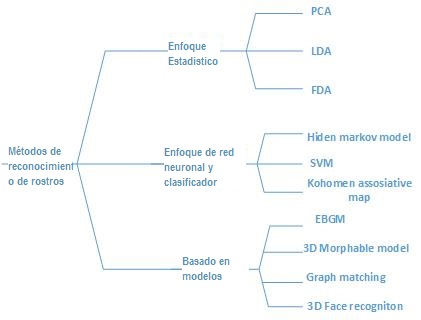
\includegraphics[scale=1]{Metodos}
\caption{Clasificación de métodos de reconocimiento de rostro por enfoque según \cite{zhao2003face}.}
\label{im:metodos}
\end{figure}

Como se observa en la Figura \ref{im:metodos} los métodos de reconocimiento de rostros pueden ser agrupados en métodos holísticos y métodos basados en características como en  \cite{tseng2003comparison} , y según \cite{zhao2003face} podemos agregar los métodos basados en inteligencia artificial y clasificadores o según \cite{parmar2014face} y \cite{pandya2013survey} pueden agregarse los métodos híbridos, pero las dos primeras clasificaciones son una constate en la literatura.

Los métodos holísticos tratan a la imagen como un todo, donde la extracción de características depende de la variación total de la información que conforma la imagen, por esta razón no sabemos que características se extraen, ni podemos darles una jerarquía de valores, esta es la razón por la cual son sensibles a cambios de iluminación y fondo. 

Este es el motivo por el cual varias de las contribuciones en estado del arte se concentran en presentar métodos holísticos robustos a esta clase de problemas como \cite{zhao1999theoretical} o nuevas forma de pre-procesamiento como \cite{gross2003image}.

Los métodos basados en modelos, también conocidos como basados en características, como lo dice su nombre se basan en formas localizadas de extracción de características o áreas localizadas de la imagen como pueden ser los ojos.
Generalmente el reconocimiento se realiza mediante una formula de distancia entre las características de dos diferentes imágenes, un buen ejemplo de ello es \ac{EBGM} en \cite{wiskott1997face} y en \cite{bolme2003elastic}.

Además \cite{zhao2003face} considera que se puede agregar a estas dos categorías un tercer enfoque basado en redes neuronal y clasificadores donde en vez de tener un formula de distancia, el reconocimiento se realiza a través de un clasificador o otro método basado en inteligencia artificial. Pero la extracción de características sigue dependiendo de una forma que puede encajar como método holístico o basado en características.

%Debido a ello para este trabajo de tesis se considera la separación de \cite{tseng2003comparison} y se usará como referencia para futuras comparaciones.
\section{Métodos holísticos}
En esta sección se hace una breve introducción a los métodos holísticos que se usan como referencia para la propuesta. Se menciona su funcionamiento general y sus principales características.


\subsection{\acf{PCA}}
\ac{PCA} es un método para la reducción de la dimensionalidad sin supervisión que puede ser aplicada para abordar el problema de reconocimiento de rostros. En \cite{sirovich1987low} se argumenta que cualquier imagen de rostro puede ser aproximadamente reconstruida como la suma con pesos de una pequeña colección de imágenes base que llaman \textit{eigenimages} y la media de las imágenes del rostro. Con ello \cite{turk1991eigenfaces} presenta su conocido método de \textit{eigenfaces}.

A continuación una breve explica como funciona este método:

Se supone que $\Gamma$ es un vector $N^2\times 1$ que corresponde a una imagen de rostro $N\times N$ llamada $I$ donde el objetivo es representar $\Gamma (\Phi-media)$ en un espacio de baja dimensión; $\Phi- media=w_1u_1+w_2u_2+.....w_ku_k$ donde $k<<N^2$ , $w$ es el peso asociado al \textit{eigenface} $u$.

Entonces si se tiene un conjunto de imágenes de rostro del mismo tamaño ${I_1,I_2,...,I_Q}$ donde cada $I_i$ se puede representar como un vector $\Gamma_i$, se tiene que calcular el vector promedio de rostro $\Psi$:
\[\Psi =\frac{1}{Q}\sum^Q_{i=1}\Gamma_i\] 
La nueva representación del rostro es: 
\[\Phi_i=\Gamma_i-\Psi\]
Después se calcula una matriz de covarianza $Co$:
\[Co=\frac{1}{Q}\sum^M_{n=1}\Phi_n \Phi^T_n=AA^T \]
Siendo una matriz $N^2\times N^2$ donde $A=[\Phi_1\Phi_2...\Phi_M]$ es una matriz $N^2\times Q$.

Sobre la matriz $AA^T$ se debe hallar auto vectores $u_i$, pero resulta ser una matriz muy grande lo que resulta poco practico, por lo que se considera la matriz $A^TA$ que es una matriz $Q\times Q$ donde si podemos calcula auto vectores $v_i$ siendo: 
\[A^TAv_i=\mu_iv_i\]
Dónde existe una relación de correspondencia donde los $Q$ autovalores y autovectores de $A^TA$ son los $Q$ autovalores y autovectores más grandes de $AA^T$. De esta manera mantenemos los $K$ vectores mas significativos. Ahora cada rostros esta representado por: 
\[\Phi_i-media= \sum^{K}_{j=1} w_j u_j, (W_j=u^T_j\Phi_i)\]
Dónde $u_j$ es un \textit{eigenface}, finalmente cada rostros puede ser representado como una colección de pesos:
\[\Omega_i=\begin{bmatrix}
w^i_1\\ 
w^i_2\\ 
...\\ 
w^i_k
\end{bmatrix} , i=1,2,...,Q\]

De esta manera \ac{PCA} reduce la dimensión de una imagen de rostro a un conjunto de pesos. Un problema que tiene esta relacionado al proceso de reducción en si donde no se sabe que características se están extrayendo y presenta una susceptibilidad a la variación de la data ingresada.

\subsection{\ac{KFA}}
\ac{KFA} \cite{liu2006capitalize} es un método que capitaliza la técnicas de incremento de la dimensionalidad, donde argumenta que métodos de reducción de dimencionalidad como \ac{PCA} tienen problemas reconociendo patrones complejos como lo es el rostro, por lo tanto es necesario un método que pueda reconocer patrones de alta dimencionalidad.

\ac{KFA} primero realiza un mapeo del espacio de la información de entrada a un espacio de características de alta dimensionalidad, y después implementa el análisis multiclase de Fisher en dicho espacio de características. \ac{KFA} usa Gabor Wavelets (en la sección \ref{scc::EBGM} se explica con más detalle) como método para incrementar la dimensionalidad.

\ac{KFA} posee varias ventajas sobre \ac{PCA} ya que su representación de la información permite una mejor distinción entre las clases que componen su espacio dimensional.

%\subsubsection{\ac{KPCA}}
%Es una forma no lineal de \ac{PCA} \cite{scholkopf1998nonlinear}, con el uso de una función integral como operador de una función Kernel, se pude computar con mayor eficiencia los componentes principales en un espacio de características. Su objetivo es presentar una forma de abordar el problema del calculo de auto valores que es necesario para poder realizar el proceso de \ac{PCA}.
%
%Obtiene ventajas sobre el típico \ac{PCA} porque puede reconocer patrones no lineales y la capacidad de adicionarle un kernel hace mas versátil a este método. Aunque \cite{scholkopf1998nonlinear} menciona que \ac{KPCA} no has ido comparado con otros métodos que analizan la información de forma no lineal.

\subsection{\acf{LDA}}
En aplicaciones aplicaciones típicas de reconocimiento de rostros tenemos vectores de imágenes de rostros de enormes dimensiones, y a pesar de ser proyectados en un sub-espacio, la dimensión de las características en varios casos son mayores a centenar, tampoco es conveniente que la dimensión del sub-espacio sea pequeña. %Este problema lleva a lo que se conoce como el fenómeno llamado \textit{dimensionality curse} que se refiere a los problemas se presentan al organizar y analizar data de alta dimensionalidad.

\ac{LDA} usado para el reconocimiento de rostros \cite{zhao1999subspace} es un método holístico que consiste en dos pasos: primero se proyecta la imagen del rostro de su representación original como vector a un sub-espacio de rostro a través de \ac{PCA}, luego usamos LDA para obtener un clasificador lineal en el sub-espacio de rostros creado. El criterio que se usa para determinar la dimensión del sub-espacio permite generar características que separan las clases a través de \ac{LDA} del total de la representación del sub-espacio.

\ac{LDA} presenta problemas relacionados a \ac{PCA} como poca tolerancia al ruido y su se obtiene datos de entrada con grandes variaciones de iluminación.

%parrafo de conclusion de seccion

En esta sección se ha descrito ejemplos de métodos holísticos de diferentes clases. Cada uno enfrenta el reconocimiento de rostros de manera diferente mediante reducción de dimencionalidad lineal, con un clasificador y con un aumento de la dimencionalidad. 

En todos ellos no sabemos que características estamos midiendo, en contraste con la  próxima sección donde presentamos un método basado en características.

\section{Basados en modelos y características}
Un enfoque para abordar el reconocimiento de rostros es mediante el uso de modelos para poder hallar características locales las cuales son pueden se ponderadas para hallar una respuesta al reconocimiento de rostros. A continuación mencionamos:

\subsection{3-D Morphable Model}
3-D \textit{Morphable Model} se utilizan para el análisis de rostros debido a las propiedades intrínsecas de los rostros en 3D que proporcionan una representación que es inmune a las variaciones intra-personales como la pose y la iluminación. 

En \cite{huang2003component} dada una imagen de entrada facial individual, un 3-D \textit{Morphable Model} puede recuperar el rostro en 3D (forma y textura) y propiedades de la escena (pose y la iluminación) a través de un proceso de adaptación. El proceso de reconocimiento se realiza mediante una comparación de características con el modelo 3D puesto en la misma posición que la imagen a identificar.


%\subsection{\acf{EBGM}}
%\ac{EBGM}  es un algoritmo de inspiración biológica para el reconocimiento de objetos en el campo de la visión computacional. Se apoya en el argumento que las características visuales utilizadas basadas en Gabor Wavelet, han probado ser un buen modelo del procesamiento visual temprano en el cerebro, más precisamente células simples en la corteza visual primaria. 

%Los objetos visuales en \ac{EBGM} se representan como grafos etiquetados, donde los nodos representan texturas locales basados en Gabor Wavelet. Así, una imagen de un objeto se representa como una colección de texturas locales en una determinada disposición espacial. 

%El reconocimiento se realiza a partir de comparaciones entre grafos para medir su parecido. Este método de reconocimiento es ampliado en la sección \ref{scc::EBGM}.

\section{Basados en redes neuronales}

La idea básica del uso de una red neuronal es adaptar la red con una entrada para cada pixel, pero como esto es una solución poco practica debido a la gran cantidad de pixeles, una solución es modificar los datos de entrada de la red a través de alguna técnica de reducción de dimensionalidad o algún método de extracción de características.

Una propuesta del uso de redes neuronales es \cite{cottrell1990face}  donde se utiliza dos redes perceptron multicapa con \textit{back propagration} donde la primera capa trabaja en modo auto asociado extrayendo características para la segunda capa donde se realiza la clasificación. Es propuesto como un método para reconocer una gran cantidad de imágenes pero el autor menciona que inclusive en buenas condiciones no mejora el desempeño en comparación a \ac{PCA}.

Otro método de reconocimiento de rostros automatizado es presentado por \cite{lin1997face}, donde utiliza una red neuronal que se basa en la toma de decisiones probabilísticas \ac{PDBNN}, consta de tres módulos, detector de rostros, detector de ojos, y reconocedor de rostros. Este método se diferencia de otros porque utiliza la zona de la cara que contiene las cejas los ojos y la nariz, pero no la boca. La boca no se considera por que presenta muchas variaciones por el cambio de expresión facial, por lo que al fin de lograr un método robusto a cambios de expresión se descarto esa zona.

Las \acf{PDBNN} tienen una característica única, que es su estructura modular. Es decir, para que se reconozca cada clase, el \ac{PDBNN} dedica una de sus sub-redes para la representación de esta clase. En comparación con la mayoría de los sistemas de reconocimiento multi-clase utilizando una función de discriminar entre dos clases, tiene \ac{PDBNN} una menor tasa de falsas alarmas-rechazo debido a que sus funciones discriminantes obedecen a una restricción probabilística.

En \cite{er2002face} se  presentó un método holístico para el reconocimiento facial, donde las características se extraen con \ac{PCA} y se utilizan como entrada para una red neuronal \ac{RBF}. Las redes \ac{RBF} tienen un buen rendimiento para los problemas de reconocimiento, tienen topología compacta y el aprendizaje es rápido. Además de las tareas de reconocimiento de rostro tradicionales  (identificación y verificación de la identidad) las redes neuronales se han utilizado para diversas tareas, tales como la identificación de género y el reconocimiento de expresiones faciales. 

\section{Consideraciones finales}
El reconocimiento de rostros es un área con una gran cantidad de trabajos y muy amplia en técnicas como se vio en este capitulo, cabe resaltar las varias formas en que la totalidad de técnicas presentadas en el estado del arte pueden ser agrupadas, ya que no existe un consenso unificado en su clasificación.

En el estado del arte aun son pocas las propuesta de llevar el reconocimiento de rostros a la vídeo vigilancia como se observa en el Capitulo \ref{chap:Intro} por ello su necesidad de proponer y probar propuestas para lograr un reconocimiento de rostros en vídeo vigilancia abordando todas las dificultades que se presenta en este tipo de escenarios donde el ambiente no es controlado.

